\documentclass{article}
\usepackage{tikz}
\usepackage{listings}
\usetikzlibrary{calc,shapes.multipart,chains,arrows}

\title{Linked Lists}


\begin{document}
\maketitle

\begin{center}
  \rule{0.5\textwidth}{0.4pt}
\end{center}

\section{Linked Lists}
\begin{itemize}
  \item{A chain of Nodes}
  \item{Each node has 2 parts, an item and a pointer}
  \item{The last pointer points to \textit{None}}
  \item{The first node is called a \textit{Head}}
\end{itemize}


\begin{center}
  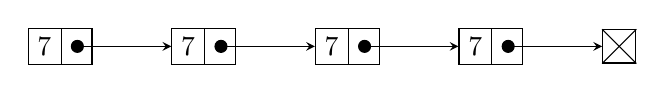
\begin{tikzpicture}[list/.style={rectangle split, rectangle split parts=2, draw, rectangle split horizontal}, >=stealth, start chain]
    \node[list,on chain] (A) {7};
    \node[list,on chain] (B) {7};
    \node[list,on chain] (C) {7};
    \node[list,on chain] (D) {7};
    \node[on chain,draw,inner sep=6pt] (E) {};
      \draw (E.north west) -- (E.south east);
      \draw (E.north east) -- (E.south west);
      \draw[*->] let \p1 = (A.two), \p2 = (A.center) in (\x1, \y2) -- (B);
      \draw[*->] let \p1 = (B.two), \p2 = (B.center) in (\x1, \y2) -- (C);
      \draw[*->] let \p1 = (C.two), \p2 = (C.center) in (\x1, \y2) -- (D);
      \draw[*->] let \p1 = (D.two), \p2 = (D.center) in (\x1, \y2) -- (E);
  \end{tikzpicture}
\end{center}

\begin{center}
  \rule{0.5\textwidth}{0.4pt}
\end{center}

\section{Linked List ADT}
\begin{itemize}
  \item{\begin{verbatim}isempty()   # is the linked list empty\end{verbatim}}
  \item{\begin{verbatim}add()       # add an item to the linked list\end{verbatim}}
  \item{\begin{verbatim}remove()    # remove an item from the linked list\end{verbatim}}
\end{itemize}

\begin{center}
  \rule{0.5\textwidth}{0.4pt}
\end{center}

\pagebreak

\section{Defining the Linked List}
\begin{lstlisting}[language=Python, frame=single]
Class Node:
    def __init__(self, item, next):
        self.item = item
        self.next = next

Class LinkedList:
    def __init__(self):
        self.head = None

    def add(self, item):
        self.head = Node(item, self.head)

    def remove(self):
        self.is_empty():
            return None
        else:
            item = self.head.item
            self.head = self.head.next
            return item

    def is_empty(self):
        return self.head == None
\end{lstlisting}

\begin{center}
  \rule{0.5\textwidth}{0.4pt}
\end{center}

\end{document}
